%==================================================================================================
\FloatBarrier
\chapter{Neural networks}

In this chapter attention will be given to artificial neural networks (ANN) which are one of most 
popular data processing models in self learning systems \cite{Abiodun2019} \cite{Tran2021}
\cite{Syed2021}. First focus will be given to biological neural networks, that will be referred 
to as a neural circuits (NC) in order to be consistent with nomenclature \cite{Purves2001} as 
well as to avoid confusion with ANN.  
After that an electrical models of NC will be shortly described and finally a mathematical models
that are used in modern ANN solutions will be discussed. Special attention will be given to 
computational complexity of both running and teaching described ANN models. 



%==================================================================================================
\FloatBarrier
\section{Basic concepts}

%--------------------------------------------------------------------------------------------------
\FloatBarrier
\subsection{Biological networks}
The subject of artificial neural networks belongs to the interdisciplinary field of research 
related to biology, electronics, mathematics, automation, and medicine.
Artificial neural networks were created based on knowledge about the functioning of the nervous
system of living creatures. 
The nerve cell, or neuron for short, is the basic component of the nervous system.
Understanding the mechanisms of operation of individual neurons and their interaction is 
particularly important for understanding the processes of acquiring, transmitting, processing,
and using information in neural networks.
For this reason, the real neuron model is extremely important. Like any other cell, a neuron has
a body called a soma, inside which is a nucleus.
From the soma of the neuron numerous connections to other cells emerge.
Two types of connections can be distinguished:
\begin{itemize}
	\item dendrites - numerous, thin, and densely branched, 
	\item axon -  single thicc forking at the end.
\end{itemize}
Input signals go to the cell via synapses, and the output signal goes through the axon
and its numerous branches called collateral.
\begin{figure}[htb] 
	\label{fig:neuron}
	\centering
	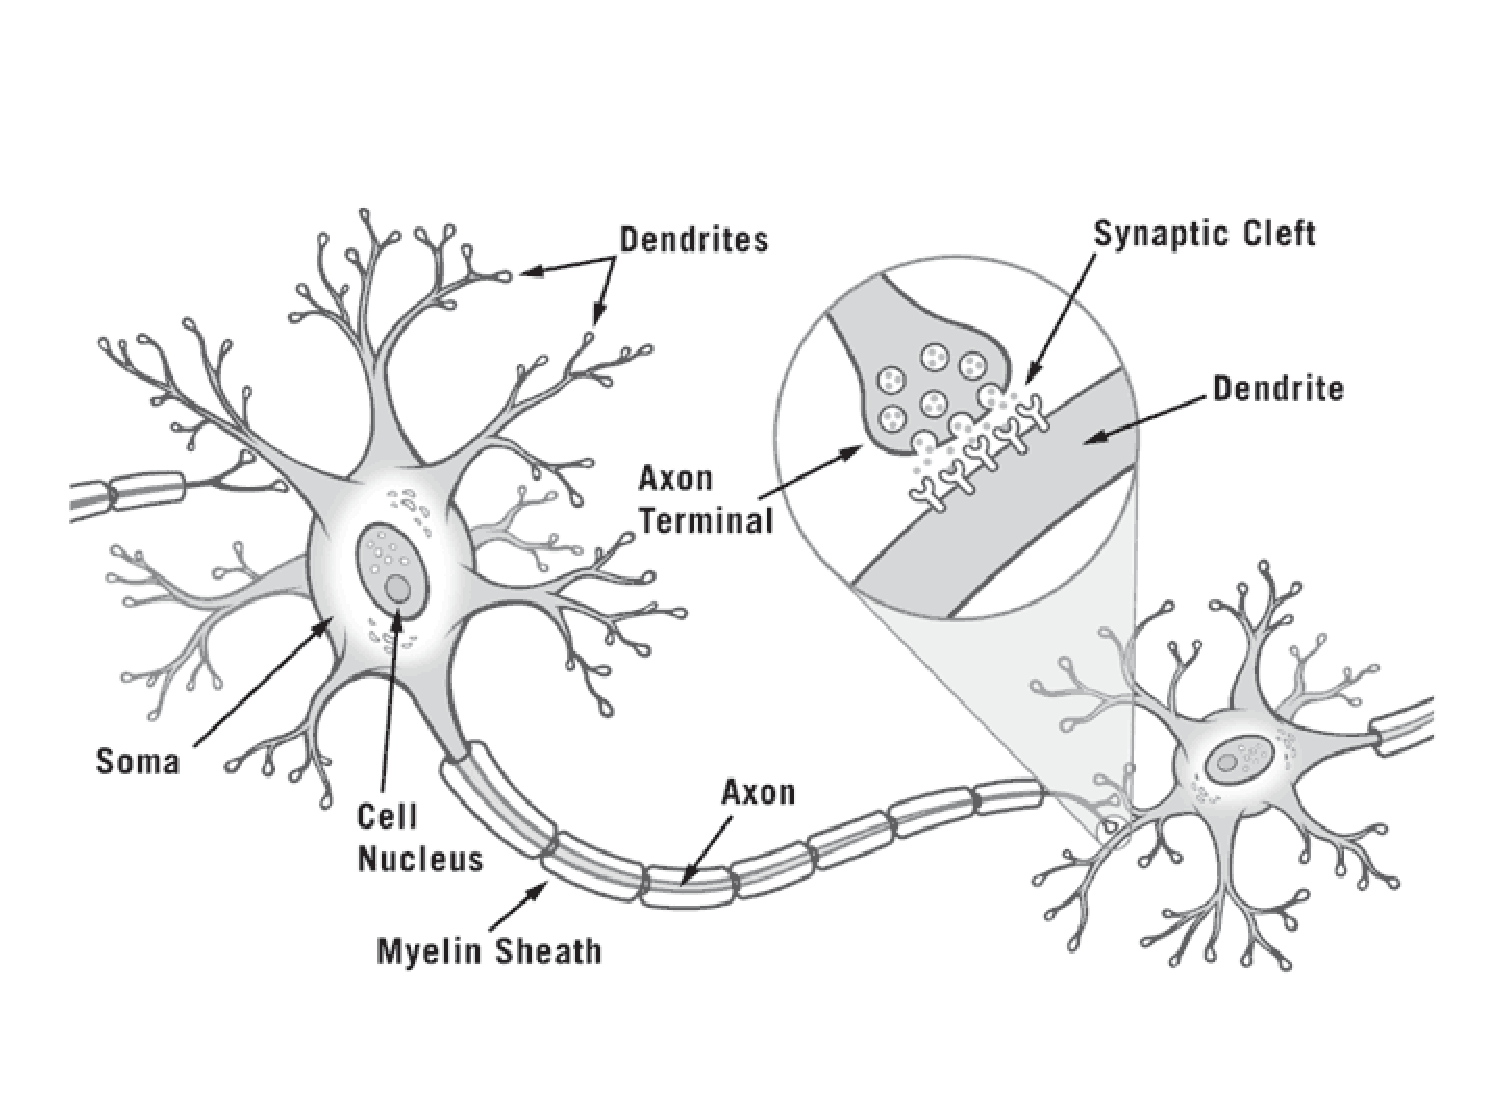
\includegraphics[width=\textwidth]{figures/neural_cell}
	\caption{Biological neuron}
\end{figure}
The collaterals reach the soma and dendrites of other neurons to form more synapses. 
Synapses that connect the outputs of other nerve cells to a given cell can therefore be found
both on the dendrites and directly on the cell body.
The transmission of signals inside the nervous system is a complex chemical-electrical process. 
In simplified terms, it can be assumed that the transmission of the nerve impulse from one cell to
another is based on the secretion of special chemical substances called neurotransmiter 
under the influence of stimuli coming from synapses.

These substances act on the cell membrane to cause a change in its electric potential, 
the change being stronger the more neurotransmiters appear on the cell membrane.
Individual synapses differ in size and the ability to accumulate neurotransmiters near the synaptic
membrane. 
For this reason, the same impulse reaching the cell's input via a specific synapse may cause a
stronger or weaker excitation of the cell than in the case of another input.
The degree of cell excitation is measured by the degree of its membrane polarization,
which depends on the total amount of neurotransmiters emitted in all synapses.
It follows that the cell inputs can be assigned numerical coefficients (weights) corresponding to 
the number of neurotransmiters isolated at one time on individual synapses.
In the mathematical model, input signals must be multiplied by these coefficients to correctly 
take into account the influence of individual input signals on the state of the nerve cell.
More information on mathematical models of neural networks are presentet in section \ref{sec:maths}
As a result of the input pulses reaching individual synapses and the release of appropriate
amounts of the neurotransmiters, specific electrical stimulation of the cell takes place.
If the electrical imbalance is minor or if the balance of excitations and inhibitions is negative,
the cell returns to its initial state by itself, and no change can be seen in its output.

If, on the other hand, the sum of stimulations and inhibitions exceeds the cell activation
threshold, the output signal increases rapidly and a characteristic shape of
the nerve impulse is formed, sent by an axon to other neurons connected to a given cell.
This signal depends on the degree of exceeding the threshold.
The cell works on the principle: all or nothing. After fulfilling his role, the neurotransmiters
are removed. The mechanism of its removal is either absorbed by the cell,
broken down, or moved beyond the synaptic area.
It stays at the same time as generating an impulse by the nerve cell the refraction
process is running.
It is a rapid increase in the cell activation threshold to the infinite value, 
as a result of which, immediately after generating the impulse, the neuron will not be able 
to generate the next one, even with strong stimulation. This state persists for some time Ar,
called absolute refraction.
\begin{figure}[htb] 
	\label{fig:bio_activation}
	\centering
	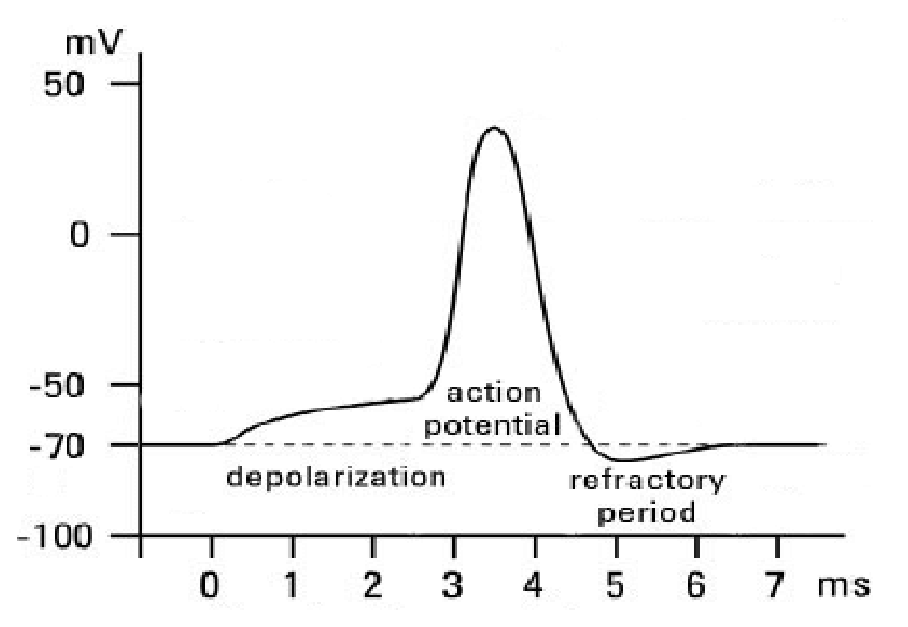
\includegraphics[width=0.6\textwidth]{figures/bio_activation}
	\caption{Response to an activation potential in neuron}
\end{figure}
This period is followed by a period of relative refraction, delta t, in which the operating
threshold returns to its resting value. In the period of At.
the cell can be stimulated, but with the use of stronger forces.
Usually in real processes the following relation Ar »At is fulfilled.

%--------------------------------------------------------------------------------------------------
\FloatBarrier
\subsection{Mathematical model of neural network}
\label{sec:maths}
Based on the principle of operation of the real neuron, a number of mathematical models were 
created that take into account, to a greater or lesser extent, the properties of 
the real nerve cell. 
The circuit diagram associated with most of these models corresponds to the McCulloch-Pitts model 
in Fig. 1.3, which includes an adder that adds weight to the input signals and a 
non-linear block that produces an output that is a non-linear function of the adder output. 
The type of the nonlinear function, in particular its continuity, has a decisive influence on 
the choice of the neuron learning technique (selection of weights). 
The second important factor is the pre-selection of the learning strategy. 
Two approaches can be distinguished here: supervised learning and unsupervised learning. 
In the teacher learning mode, it is assumed that the desired output signal of the neuron 
(destination d,) is known, and the selection of weights must be carried out in such a way that the 
current output signal of the neuron y is closest to the set value d. 
An important element here is the knowledge of the desired value of d, of the neuron output. 
If we are unable to provide this, it remains to choose a learning strategy without a teacher. 
The selection of weights then takes place on a different basis, either by using the competition of 
neurons with each other (Winner Takes All strategy) or by using the Hebb learning method. 
In teaching without a teacher, at the stage of teaching the neuron, we are not able to predict the 
output signal of the neuron, unlike the mode with the teacher, where the learning result 
is predetermined by the choice of learning values. 

%==================================================================================================
\FloatBarrier
\section{Representation in computer}

%==================================================================================================
\FloatBarrier
\section{Learining algorithms}

%==================================================================================================
\FloatBarrier
\section{Evolutionary algorithms}

%--------------------------------------------------------------------------------------------------
\FloatBarrier
\subsection{Overwiew}
Genetic algorithms are methods of solving various problems, mainly optimization problems, 
based on evolution. 
They mimic the natural process of evolution that involves genetic changes occurring in populations 
of living organisms over time. 
The main factor of evolution is natural selection, which makes it possible that among genetically 
different individuals of a population they survive and leave only the offspring best adapted to 
the environment. 
Genetic algorithms perform simulated evolution on the so-called chromosomes, consisting of genes.
The gene values are alleles. In the classic (basic) genetic algorithm, chromosomes are binary 
sequences with alleles equal to 0 or 1. 
Individuals of the population (chromosomes) are assessed utilizing an appropriately defined fitness 
function. 
In genetic algorithms, we distinguish a selection stage that selects individuals with the highest 
value of the adaptation function to the parental population (parental pool) from the current 
chromosome population. 
The next step is to use genetic operators, such as crossing and mutation, to recombine genes 
in the chromosomes. 
The operation of crossing is the exchange of fragments of parents' chromosomes. Parent pairs to be 
crossed are selected randomly from the parent pool with a defined probability of crossing. 
After the crossing operation, the parents in the parent pool are replaced with their descendants. 
The mutation operation changes the values of genes in the chromosomes according to the given 
probability p. 
This means that the values of the genes selected in this way are changed from 0 to 1 or 
vice versa. 
The p-value is usually very small, so a small number of chromosomes undergo such changes.


%--------------------------------------------------------------------------------------------------
\FloatBarrier
\subsection{Operators}
Figure \ref{fig:genetic_algorithm} shows the flowchart on which the genetic algorithm works.
There are 7 essential steps that will now be discussed in sequence.

\begin{figure}[htb] 
	\centering
	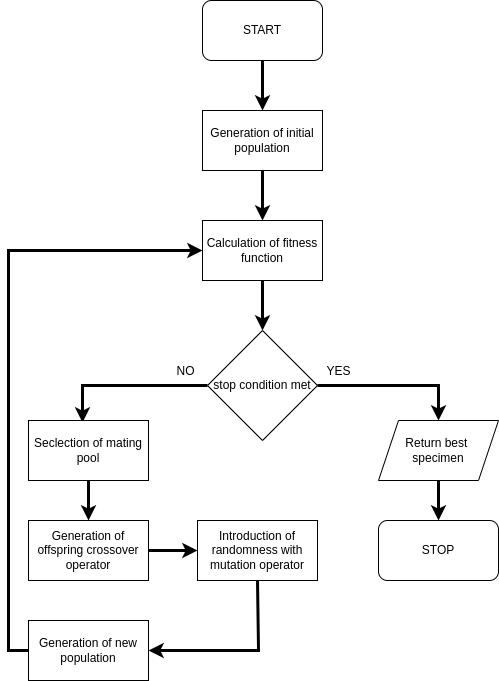
\includegraphics[width=\textwidth]{figures/genetic_algorithm}
	\caption{Overwiew of genetic algorthm}
	\label{fig:genetic_algorithm}
\end{figure}

\FloatBarrier
\subsubsection{Selection of the initial population} 
Establishing an initial population is the first step in the genetic algorithm. 
It consists of the deliberate selection of the desired number of chromosomes (individuals), 
i.e. chains - ordered sequences of genes - of a certain length.

\subsubsection{Assessment of the chromosome adaptation}
Each chromosome in the population is assessed based on an appropriately defined fitness 
function. 
In the classical (basic) genetic algorithm, the greater the value of this function, 
the better the chromosome and its better adaptation. The form of the adaptation function 
depends on the type of problem to be solved. 
In the classical algorithm, it is assumed that the adaptation function always takes 
non-negative values and that The optimization problem is the task of searching for the 
maximum of this function If the original form of the adaptation function does not meet 
these assumptions, the appropriate transformation is carried out (eg the problem of finding 
the minimum of the function can be easily reduced to the problem of searching for the maximum). 

\subsubsection{Checking the stop condition of the algorithm} 
The determination of a stop condition for a genetic algorithm depends on the specific algorithm. 
In optimization problems, if the maximum (or minimum) value of the fitness function is known, 
the algorithm may be stopped after the desired optimal value has been obtained, possibly with 
a specified accuracy. 
You can also stop the algorithm if continuing to run it does not improve the best value 
already obtained. 
It can also be stopped after a certain run time or after a certain number of iterations. 
If the stop condition is met, it goes to the last step, which is the derivation of the best 
chromosome. If not, the next step is selection.

\subsubsection{Chromosome selection} 
As mentioned before, the selection consists in selecting from the current chromosome population into 
the parental population, the individuals of which are then crossed and mutated to form a new 
population of descendants. 
The basic selection method used in the classical genetic algorithm is the roulette method, 
but other methods are also used, such as a tournament or ranking selection. 
We will now introduce the above-mentioned methods. 

\paragraph{Roulette algorithm} 
Chromosome selection consists in selecting, based on the value of the fitness function 
(calculated in step 2), those chromosomes that will be involved in creating descendants for 
the next generation, i.e. the next generation. 
This selection is carried out following the principle of natural selection, i.e. the 
chromosomes have the greatest chance of participating in the creation of new individuals
with the highest value of fitness function. The most famous selection method is the roulette 
wheel selection method, which owes its name to the analogy of drawing with a roulette wheel. 
It is used in the classical (basic) genetic algorithm. In this method, each chromosome is 
assigned a segment of a roulette cat with a size proportional to the value of the adaptation 
function of a given chromosome. 
Thus, the greater the value of the adaptation function, the larger the sector (sector) on 
the roulette wheel. 
The entire roulette wheel corresponds to the sum of the values of the fitness function of 
all chromosomes of the population under consideration. For each chromosome, 
specimen $s$ in population $\mathfrak{B}$ size, the corresponding segment of the 
circle $P(s)$ is part of the whole circle expressed according to the following formula:
\begin{equation}
	P(s) = \frac{F(s)}{\sum_{s \in \mathfrak{B}}F(s)}
\end{equation}
wherein F (ch.) is the value of the chromosome adaptation function ch, p. (ch) is 
the selection probability of the ch chromosome. 
Choosing a chromosome can be viewed as spinning the roulette wheel, with the result that
the chromosome belonging to the roulette wheel segment thus drawn wins (selected). 
Obviously, the larger the wheel segment, the more likely it is to win the corresponding 
chromosome. 
Thus, the probability of selecting a given chromosome is greater, the greater the value 
of its fitness function. 
If we treat the entire circle of the roulette wheel as the numerical interval [0, 100], 
then the random selection of the chromosome can be treated as a random selection of a 
number from the range $[a, b]$, where a and b mean, respectively, the beginning and the 
end of the circle segment corresponding to this segment of the circle. 
 of course, $0 \leq a < b \leq 100$. Then the drawing with the roulette wheel is reduced to a 
 random selection of a number from the range $[0,100]$, 
 which corresponds to a specific point on the roulette wheel. 
 As a result of the selection process, a parental population is created, also known as 
 a mating pool, with a size equal to N, i.e. the same as the size of the current population.

\paragraph{Tournament selection}

In tournament selection, the individuals of the population are divided into subgroups, 
and then from each of them, the individual with the best adaptation (with the highest 
value of the fitness function - step 2) is selected. 
There are two different ways of making such a selection: deterministic tournament
selection and stochastic tournament selection. In the case of a deterministic 
selection, the probability is equal to me, and in the case of a random selection, 
the probability is less than 1. 
The subgroups can be of any size, most often the population is divided into subgroups 
consisting of two or three individuals. The tournament method is suitable for both 
maximization and function minimization problems. In addition, it can be easily 
extended to tasks related to multi-criteria optimization, i.e. optimization of several 
functions at the same time. 
In the tournament method, you can change the size of the subgroups into which the 
tournament size is divided. 
Research shows that the tournament method works better than the roulette method. 
It is most often used in practice.

\paragraph{Ranking selection} 
In ranking selection, the individuals of the population are arranged 
sequentially according to the value of their fitness function. 
This can be imagined as a ranking list of individuals ranked from best to worst 
(or vice versa), where each individual is assigned a number denoting its order on 
the list and called a rank. 
The number of copies of each individual, placed in the parent pool, is set 
according to a predefined function depending on the rank of the individual. 
The advantage of the ranking method is that it can be used both to maximize and 
minimize functions. It also does not encounter the problem of premature convergence, 
which can occur when using the roulette method.

\subsubsection{The crossover operator}
The first step in crossing is selecting chromosome pairs from the parent population 
(parent pool) of a temporary population of chromosomes selected by selection and 
destined for further processing with crossing and mutation operators to form a new 
descendant population. At this stage, the chromosomes from the parental population 
are matched in pairs. This is done randomly, according to the probability of p 
crossing. 
Then, for each pair of parents selected in this way, the position of the gene 
(locus) in the chromosome is drawn, which determines the so-called crossing point. 
If the chromosome of each parent consists of L genes, then of course the crossing point 
is a natural number smaller than L. 
Therefore, the choice of the crossing point comes down to drawing a number from the 
interval [1, L-1]. 
As a result of crossing a pair of chromosomes in the body, the following pair 
of descendants is obtained: - descendant 1 - chromosome consisting of genes at 
positions 1 to 1 coming from the first parent and subsequent genes, from positions 
1 + 1 to L. coming from the second parent. - descendant 2 - chromosome consisting of 
genes in positions 1 to 4 from the second parent and subsequent genes, from position 
1, + 1 to L, from the first parent. 
A modification of the so defined one-point crossing is also used, namely a two-point 
cross over. It differs from single-point crossing in that descendants inherit fragments
of randomized crossing points. There is also a multiple-point crossover, which is a 
generalization of the previous operations, characterized by a correspondingly greater 
number of crossing points.

\subsubsection{Mutation operator}
The mutation operator, according to the probability of mutation, changes the value 
of the gene in the chromosome to the opposite (ie from 0 to 1 or from 1 to 0). 
For example, if the mutation in the following chromosome [101010011010] has a 
gene at position 9, its value of 1 changes to 0, and we obtain a chromosome 
[101010010010]. 
As mentioned before, the probability of a mutation is usually very small and 
of course, it depends on whether a given gene in a chromosome is mutated or not. 
Performing a mutation in accordance with the probability p. 
Consists, for example, in drawing a number from the interval [0, 1] 
for each gene and selecting for mutation those genes for which the drawn number 
is lower or equal to the probability p

\subsubsection{Create a new population}
Individuals obtained by the action of the genetic operators on the diseases of the 
temporary parental population are included in the new population. 
This population becomes the so-called current population for a given iteration of 
the genetic algorithm. 
In each subsequent iteration, values of the fitness function of each of the 
chromosomes of that population are computed. 
Then the stop condition of the algorithm is checked and either the result in 
the form of the chromosome with the highest value of the fitness function is derived 
or the next step of the genetic algorithm, i.e. selection, is passed. 
In the classical genetic algorithm, the entire previous chromosome population is 
replaced by an equally large new population of descendants. 
Sometimes the so-called elitist strategy consists in protecting the best 
chromosomes in subsequent iterations. 
In the classical genetic algorithm, the best-adapted individuals do not always 
pass to the next generation. 
The elite strategy is used to prevent the loss of such an individual. 
It is always included in a new population. Another modification of the classical 
genetic algorithm is the partial population replacement genetic algorithm, also 
known as the steady-state algorithm, which is characterized by the fact that 
part of the population passes to the next generation without any changes. 
This means that this part of the population is not subject to crossing and mutation 
operations. 
Often, in a specific implementation of this type of algorithm, only one or
individuals are replaced at a time instead of crossing and mutating within
the entire population. The next iteration in the genetic algorithmic is called 
generation a new generation or generation of descendants is also referred to as 
the newly created population of individuals.

\subsubsection{Derivation of the best chromosome} 
If the condition of stopping the genetic algorithm is met, the result of the 
algorithm's operation should be derived, i.e. a solution to the problem should 
be provided. 
In the classical genetic algorithm, the best solution is chromo som with the highest 
value of the fitness function.

\subsection{Chromosome coding methods} 

\subsubsection{Binary encoding}
A very important issue in genetic algorithms is the choice of chromosome representation 
(binary or other, e.g. realists) and the problem of coding potential solutions in the 
form of chromosomes. 
The classical genetic algorithm uses binary representation and decimal coding in the 
binary system, where each bit of the binary code corresponds to the next power of 2. 
For example, the binary sequence $[10001]$ is the code of the number 17, because
\begin{equation}
	1\dot 2^4 + 0\dot 2^3 + 0 \dot 2^2 + 0\dot 2^1 + 1\dot 2^0 = 17
\end{equation}

\subsubsection{Logarithmic encoding}
In order to reduce the length of chromosomes, the so-called logarithmic coding. 
It is mainly used in optimization problems with many parameters and large search spaces. 
In logarithmic encoding, the first bit (a) of the code string is the sign bit of the 
exponential function, the second bit (B) is the sign bit of the exponent, 
and the remaining bits (bin) are the representation of the exponent of the exponential function:
\begin{equation}
	[a\dot b\dot bin] = (-1)^b e^{(-1)^{a}[bin]_{10}}
\end{equation}
where $[bin]_{10}$ is the decimal value of the binary encoded number. 

\subsubsection{FLoating point encoding}

%==================================================================================================
\FloatBarrier
\section{Neuroevolution for agumented topologies}
NeuroEvolution of Augmenting Topologies (NEAT) is a genetic algorithm based on the use of three 
key techniques: tracing the history of genes, applying species division, and developing the 
topology of a neural network. 
In NEAT, genetic coding is used to record information about the structure of the neural network. 
It was designed in such a way as to allow easy assembly of genes during crossbreeding. 
Genomes are a linear representation of a neural network. Each genome is made up of two lists, 
one representing the genes for the nodes of the network and the other representing the 
genes for existing connections between the nodes. Node genes provide information about network 
entrances, nodes in the hidden layer, and network exit. 
Each of the connection genes contains information about the nodes between which the connection 
exists, the connection weight value, whether the connection is active or not, 
and has an identification number assigned. 
Mutations in the NEAT algorithm can change both the value of the weight of a given connection and 
the structure of the network. 
There are two possibilities for mutating the network structure by adding a link and by adding 
a node. 
When a link is added, a new link gene is created with a random weight value that connects the 
two nodes that did not have a link between them. 
In the case of a node addition mutation, the existing connection is split and the new node is put 
in place of the old connection, which is deactivated (this information is included in 
the connection genes). 
As a result, two new connections are added to the genome. 
The link leading to the new node is assigned a weight value of 1, and the link originating from 
the new node is assigned the weight value of the old link. 
Mutations cause genes to expand and the size of genes in a population varies. 
This fact requires an appropriate approach to the process of interbreeding of individuals from the 
population. During the process of evolution, information is gathered that tells us what genes 
correspond to genes from other individuals in a topologically diverse population. 
This information tells us the origin of each gene, so we can determine from which ancestor the 
gene was inherited. 
When a new gene is created (previously non-existent link), the Global Identification Number is 
increased and assigned to that gene. 
Hence the identification numbers represent the chronology of the emergence of new genes. 
In the case of a cross between two genomes, the descendant inherits the same identification numbers
corresponding to each gene, these numbers never change, thanks to which we have the opportunity 
to learn the history of the formation of a given unit. 
During the crossing process, genes with the same identification numbers are paired, 
they are called corresponding genes. 
Those that do not match are disjoint or redundant (depending on whether their numbers are 
within the range of the numbers of the other parent) 
If, when matching the connection genes, the given parent 'A' gene does not match the parent 'B' 
gene and the identification number of this gene is smaller from the largest parent identification 
number 'B' such a gene is disjoint. 
If the parent 'A' has non-corresponding genes and their numbers are greater than the largest gene 
number of the parent 'B', they are called redundant genes. 
Disjoint and redundant genes represent a structure that is not part of the other genome. 
When matching genes during crossbreeding, matching genes are inherited randomly 
(a gene with the same ID number is inherited from either parent 'A' or parent 'B'), 
while disjoint and redundant genes are inherited from the parent whose adjustment function results 
are greater. 
The result of the emergence of new genes and the crossing of units with different structures is 
the building of a topologically diverse population. Since entities with a smaller structure 
optimize faster than larger ones, and the fact that enlarging the network with nodes and 
connections usually lowers the result of the alignment function, newly developed structures have 
little chance of survival. 
It also results from the fact that topological diversity in the population will not be maintained. 
As a consequence, individuals with innovative changes in the structure, which in the future could 
turn out to be very positive for the course of evolution, will die out.

To maintain the diversity of the population in terms of topology, a division into species has been 
introduced, in which individuals compete with each other, having time to optimize and improve 
their structures within a given niche. 
Units are allocated to species based on their similarity in structure. 
The similarity is determined by the number of disconnected and redundant genes. 
The more disjoint genes there are, the fewer individuals are related, and therefore 
less compatible. The measure of agreement is calculated from the formula in which E 
is responsible for the number of redundant genes, D is disjointed, and the average of the 
difference in weight of the corresponding genes. 
The coefficients c1, c2, c3 are responsible for the significance of these parameters, 
N is responsible for normalization, when both genomes consist of less than 20 genes, N can be 1. 
The calculated compliance distance is compared with the established compliance threshold, 
if the threshold is exceeded, the unit is not classified into a given species. 
At each generation, genomes are allocated to species, each unit is compared in terms of 
compliance with the representatives of the species. The units representing the species are 
randomly selected genomes from the previous generation. 
If an entity from the current generation is not compatible with any existing species, 
a new species is created, so that unit becomes the representative of that species. 
In the case of genetic algorithms, as population diversity disappears, there is a tendency to 
converge to one solution, this is called genetic drift. 
To counteract this, when assigning an individual to a species, its adjustment function result is 
adjusted based on the results of the individuals in that species. 
Consequently, a given species does not make up the majority of the population, and therefore the 
entire population will not be assigned to one species. 
An important feature of the NEAT algorithm is maintaining population diversity, but the structure 
of the generated solutions is also very important in the context of the final solution. 
The ultimate goal of this model is to strive for the most optimal result. 
This is done by minimizing the dimensionality in the space of the solutions sought, therefore, 
when creating the base population, units with hidden layers are not generated. 
During the process of evolution, when mutations take place, only those structures that have a 
positive effect on the results obtained survive.
